\subsection{Estimated Combining Functions}

We next report estimates of the proportion of beneficial effects by block and overall.\footnote{We consider a total of 95 outcomes that we classify in Appendix~\ref{appendix:results}. These are the outcomes that most clearly relate to the treatment offered by the program.} The analysis is based on treatment effect \eqref{eq:effect}. Figure~\ref{fig:ppositive} displays the results from this analysis: ABC/CARE positively impacted a large percentage of the outcomes. We show the counts for treatment compared to the next best alternative chosen by parents in Figure~\ref{fig:ppositivenb}. Proportionately more outcomes are beneficial for females, but the proportions are high for both groups and well above the benchmark of 1/2. In Tables~\ref{table:abccare_rslt_pooled_counts} to \ref{table:abccare_rslt_female_counts_n10a10} of Appendix~\ref{appendix:results}, we document a large and precisely determined fraction of beneficial treatment effects well above one half for both genders for categories of outcomes spanning the life cycle through the mid 30's.

Using an $\alpha$-level of significance, one would expect to find that $\alpha\%$ of the treatment effects are ``statistically significant,'' even if the null hypothesis of no effect of the program is true simply by chance. At a 10\% level of significance, $46\%$ are statistically significant for females and $28\%$ for males (see Figure~\ref{fig:ppositive10}).

Figures~\ref{fig:ppositivehome} and Figure~\ref{fig:ppositivealternative} adjust the count in Figure~\ref{fig:ppositivenb} to analyze more clearly defined counterfactuals: treatment compared to staying at home and treatment compared to alternative preschool. These comparisons indicate that girls and boys benefit differently from alternatives to high quality treatment. Compared across all categories, girls benefit more from treatment when compared to staying at home (as opposed to attending alternative childcares), while males benefit more from treatment when compared to attending an alternative childcare arrangement (as opposed to staying at home).

\begin{sidewaysfigure}[!htbp]
\centering
\caption{Positively Impacted Outcomes, ABC/CARE Males and Females}\label{fig:ppositive}
\begin{subfigure}[h]{0.4\textwidth}
		\centering
		\caption{Treatment vs. Next Best} \label{fig:ppositivenb}
		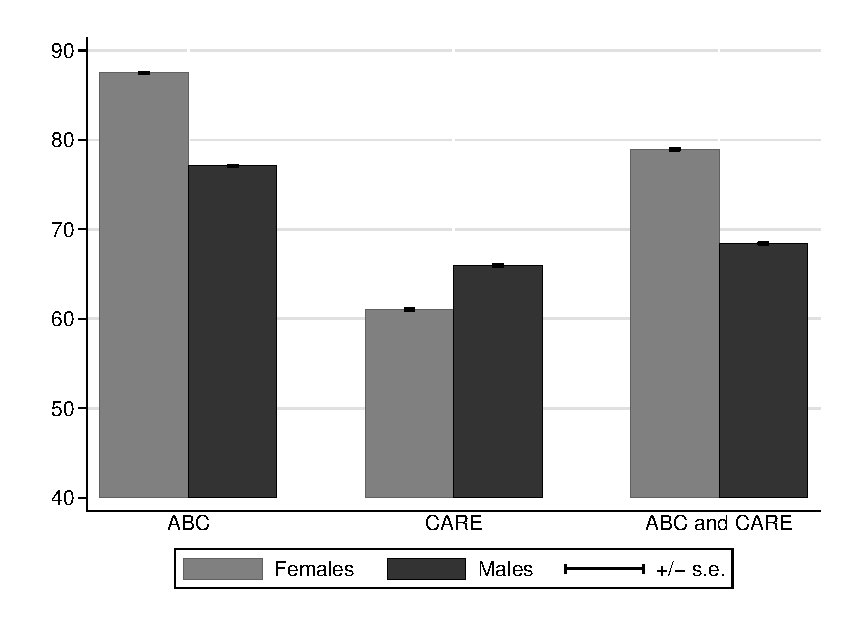
\includegraphics[width=\textwidth]{output/itt_noctrl_all.eps}
\end{subfigure}%
\begin{subfigure}[h]{0.4\textwidth}
	\centering
	\caption{Treatment vs. Next Best, Significant at 10\% Level} \label{fig:ppositive10}
		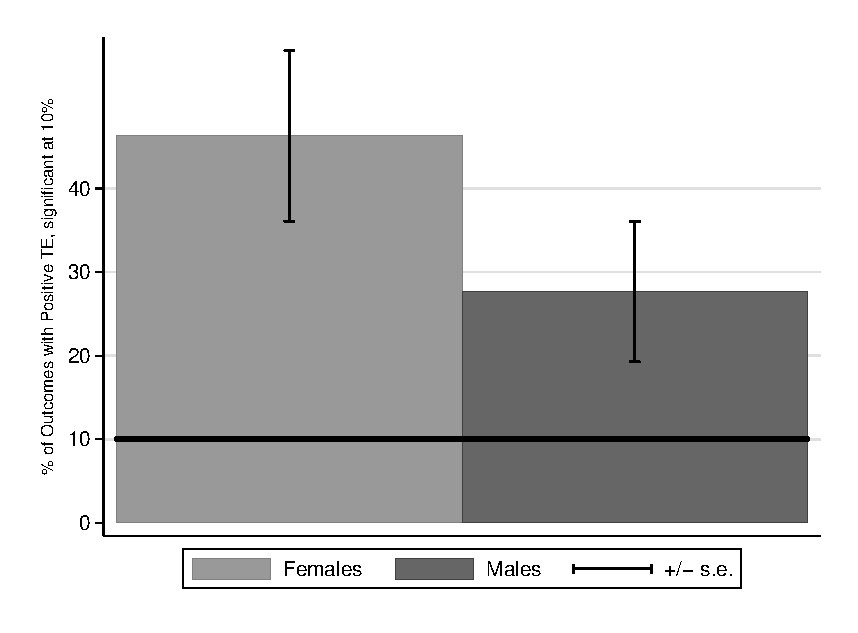
\includegraphics[width=\textwidth]{output/itt_noctrl_all_sig10.eps}
\end{subfigure}
\begin{subfigure}[h]{0.4\textwidth}
		\centering
		\caption{ Treatment vs. Stay at Home} \label{fig:ppositivehome}
		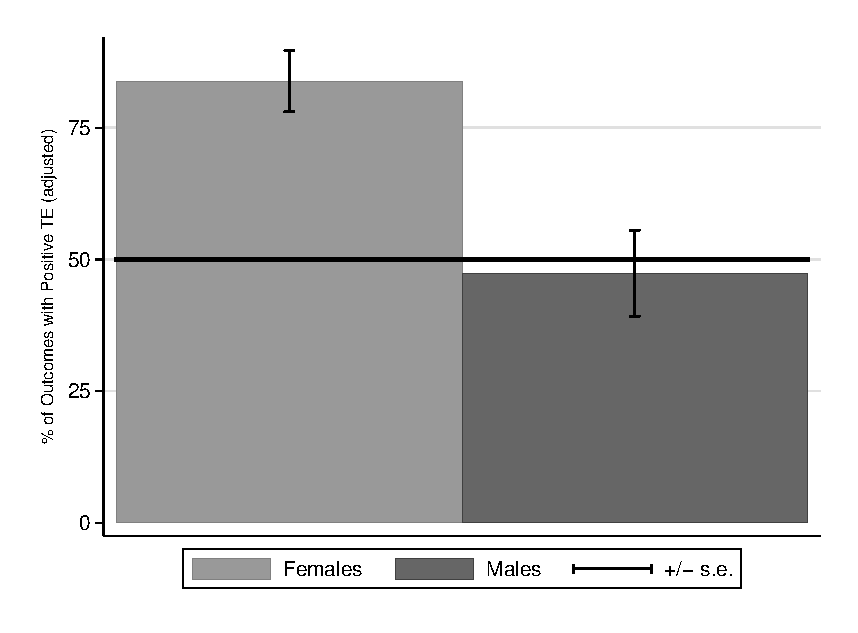
\includegraphics[width=\textwidth]{output/epan_ipw_p0_all.eps}
\end{subfigure}%
\begin{subfigure}[h]{0.4\textwidth}
	\centering
	\caption{Treatment vs. Alternative Preschool} \label{fig:ppositivealternative}
		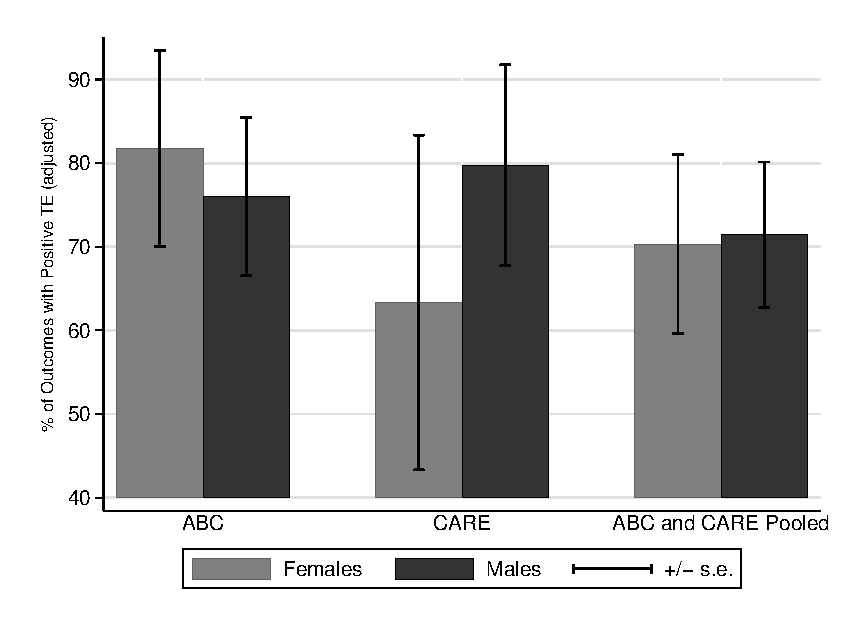
\includegraphics[width=\textwidth]{output/epan_ipw_p1_all.eps}
\end{subfigure}
\scriptsize \justify
Note: Panel (a) percentage of outcomes displaying a positive treatment effect, comparing treatment to next best. Panel (b) percentage of outcomes displaying a positive and statistically significant treatment effect (10\% significance level). Panel (c) displays the percentage of outcomes with a positive treatment effect, comparing treatment to staying at home. Panel (d) displays the percentage of outcomes with a positive treatment effect, comparing treatment to alternative childcare arrangements. Standard errors are based on the empirical bootstrap distribution. For Panel (b) we perform a ``double bootstrap'' procedure to first determine significant treatment effects at $10\%$ level and then calculate the standard error of the count.\\
\end{sidewaysfigure}
